\documentclass{article}
\usepackage{amsmath}
\usepackage{graphicx}
\usepackage{geometry}
\begin{document}

\section{Stratified Test Problem}
Note: I will be using the variable $m=\rho_0 u$. The variable $u$ does not exist in the discrete formulation. A quotient $m / \rho_0 (= (\rho_0 u)/\rho_0 )$ can not be simplified to $u$.
\subsection{Continuous Formulation}
As Poisson bracket we take 
\begin{equation}
	\label{sntc:eq:contPoiBra}
\left\{\mathcal{F}, \mathcal{G}\right\} = \int_\Omega \! \frac{\delta \mathcal{G}}{\delta p} \rho_0 \frac{\partial}{\partial x} \frac{\delta \mathcal{F}}{\delta m} - \frac{\delta \mathcal{F}}{\delta p} \rho_0 \frac{\partial}{\partial x} \frac{\delta \mathcal{G}}{\delta m} \, \mathrm{d}x.
\end{equation}
As Hamiltonian we take
\begin{equation}
	\mathcal{H} = \int_\Omega \! \frac{1}{2} \frac{1}{\rho_0} \left( m^2 + p^2 \right) \, \mathrm{d}x.
\end{equation}
The background density can be a function of x: $\rho_0=\rho_0(x)$.

Substituting the Hamiltonian into the Poisson brackets yields 
\begin{equation}
	\begin{aligned}
		\frac{\partial m}{\partial t} &= -\frac{\partial p}{\partial x}, \\
		\frac{\partial p}{\partial t} &= - N^2 m - \frac{\partial m}{\partial x}, \\ 
		N^2 &= -\frac{\partial \rho_0/\partial x}{\rho_0}.
	\end{aligned}
\end{equation}

We choose a domain $\Omega = [0,1]$ with solid wall boundary conditions. Choosing an exponential background density, yields a constant $N^2$ and we can find an exact solution using separation of variables,
\begin{equation}
	\begin{aligned}
		m &= e^{-\frac{1}{2} N^2 x} \sin(2 \pi k x) \sin(2 \pi \sigma t), \\
		p &= e^{-\frac{1}{2} N^2 x} \left[\frac{N^2}{4\pi\sigma} \sin(2 \pi k x) + \frac{k}{\sigma} \cos(2 \pi k x)\right] \cos(2 \pi \sigma t),
	\end{aligned}
\end{equation}
with dispersion relation
\begin{equation}
	4 \pi^2 \sigma^2 = \frac{1}{4} N^4 + 4 \pi^2 k^2.
\end{equation}

\subsection{Discretization}
We triangulate our domain into lines segments $K$ of length $\Delta x$. We number the elements: The first element is element 1, the second element is element 2, $\hdots$, the last element is element $N$. The elements have boundaries $e$. The left (outer) boundary of element 1 is boundary 1, the (inner) boundary between element 1 and 2 is boundary 2, $\hdots$, the right (outer) boundary of element $N$ is boundary $N+1$.

We introduce the discrete variables $m_h$ and $p_h$, which are approximations to the continuous $m$ and $p$. Our interim Poisson brackets follows from (\ref{sntc:eq:contPoiBra})
\begin{equation}
	\left\{\mathcal{F}, \mathcal{G}\right\} = \sum_K \int_K \! \frac{\delta \mathcal{G}}{\delta p_h} \rho_0 \frac{\partial}{\partial x_h} \frac{\delta \mathcal{F}}{\delta m_h} - \frac{\delta \mathcal{F}}{\delta p_h} \rho_0 \frac{\partial}{\partial x_h} \frac{\delta \mathcal{G}}{\delta m_h} \, \mathrm{d}K.
\end{equation}
For each element the integral holds and $\partial/\partial x_h$ means integration with respect to $x$ on each element. The question is: What to do with $\rho_0$ in this formulation: Do we treat it as an continuous variable, $\rho_0 = \rho_0(x)$, or as an discrete variable, $\rho_0 = \rho_{0_h}$? For now, we keep both options open.

To introduce a numerical flux we integrate by parts
\begin{equation}
	\label{sntc:eq:intPoiBra}
	\begin{aligned}
\left\{\mathcal{F}, \mathcal{G}\right\} &= \sum_K \int_K \! -  \frac{\delta \mathcal{F}}{\delta m_h} \frac{\partial}{\partial x_h} \left( \rho_0 \frac{\delta \mathcal{G}}{\delta p_h} \right) + \frac{\delta \mathcal{G}}{\delta m_h} \frac{\partial}{\partial x_h}  \left( \rho_0  \frac{\delta \mathcal{F}}{\delta p_h} \right)  \, \mathrm{d}K \\
&+ \sum_K \int_{\partial K} \! \frac{\delta \mathcal{G}}{\delta p_h} \rho_0 \hat{n} \scalebox{2}{$\widehat{\scalebox{0.725}{$\frac{\delta F}{\delta m_h}$}}$} - \frac{\delta \mathcal{F}}{\delta p_h} \rho_0 \hat{n} \scalebox{2}{$\widehat{\scalebox{0.725}{$\frac{\delta G}{\delta m_h}$}}$} \, \mathrm{d}\Gamma,
	\end{aligned}
\end{equation}

where $\partial K$ is the boundary of line segment $K$ and $\Gamma$ the surface integral (or point integral since we are in 1D). $\hat{n}$ is the outward normal (= plus or minus one). The wide hat indicates a numerical flux. To ensure anti-symmetry, we choose as numerical flux
\begin{equation}
	\begin{aligned}
		\scalebox{2}{$\widehat{\scalebox{0.725}{$\frac{\delta G}{\delta m_h}$}}$} = (1-\theta) \frac{\delta G}{\delta m_h^L} + \theta \frac{\delta G}{\delta m_h^R}, \\
		\scalebox{2}{$\widehat{\scalebox{0.725}{$\frac{\delta F}{\delta m_h}$}}$} = (1-\theta) \frac{\delta F}{\delta m_h^L} + \theta \frac{\delta F}{\delta m_h^R}, 
	\end{aligned}
\end{equation}
where the superscript $L$ indicates the element to the left of a boundary and the superscript $R$ indicates the element to the right of a boundary. Since we are on a line segment in one dimension, there is no confusion on what left and right means. At a solid wall boundary, we have
\begin{equation}
	m (x=0,1) = 0 \Rightarrow \frac{\delta H}{\delta m}(x=0,1) = 0 \Rightarrow \scalebox{2}{$\widehat{\scalebox{0.725}{$\frac{\delta H}{\delta m_h}$}}$}(x=0,1) = 0.
\end{equation}
By anti-symmetry we also require $\scalebox{2}{$\widehat{\scalebox{0.725}{$\frac{\delta F}{\delta m_h}$}}$}(x=0,1) = 0$. The numerical flux along the outer boundaries is zero. The integration along the boundary in the summation over all elements in (\ref{sntc:eq:intPoiBra}) visits all internal boundaries twice, and rewriting the summation over all elements into a summation over all internal boundaries and working out the brackets in yields
\begin{equation}
	\label{sntc:eq:ibtPoiBra}
	\begin{aligned}
\left\{\mathcal{F}, \mathcal{G}\right\} &= \sum_K \int_K \! \left(\frac{\delta \mathcal{G}}{\delta m_h}\frac{\delta \mathcal{F}}{\delta p_h} - \frac{\delta \mathcal{F}}{\delta m_h}  \frac{\delta \mathcal{G}}{\delta p_h} \right) \frac{d \rho_0}{d x_h}   \, \mathrm{d}K \\
&+ \sum_K \int_K \! - \frac{\delta \mathcal{F}}{\delta m_h} \rho_0  \frac{\partial}{\partial x_h} \frac{\delta \mathcal{G}}{\delta p_h} + \frac{\delta \mathcal{G}}{\delta m_h} \rho_0 \frac{\partial}{\partial x_h} \frac{\delta \mathcal{F}}{\delta p_h}  \, \mathrm{d}K \\
&+ \sum_{e \in \Gamma_i} \int_{e} \! \left(\frac{\delta \mathcal{G}}{\delta p_h^R} \rho_0^R - \frac{\delta \mathcal{G}}{\delta p_h^L} \rho_0^L \right) \left[  (1-\theta) \frac{\delta F}{\delta m_h^L} + \theta \frac{\delta F}{\delta m_h^R}\right] \\
& \quad \qquad - \left(\frac{\delta \mathcal{F}}{\delta p_h^R} \rho_0^R - \frac{\delta \mathcal{F}}{\delta p_h^L} \rho_0^L \right) \left[  (1-\theta) \frac{\delta G}{\delta m_h^L} + \theta \frac{\delta G}{\delta m_h^R}\right] \, \mathrm{d}\Gamma,
	\end{aligned}
\end{equation}	
where $\Gamma_i$ are all internal boundaries. On $\rho_0$: If $\rho_0$ is treated as an continuous variable, $\rho_0^L = \rho_0^R$ for each boundary and $d \rho_0/d z$ is nonzero. If $\rho_0$ is treated as an discrete variable, then $\rho_0^L \neq \rho_0^R$ for each boundary and $d \rho_0/d z$ is zero.

On each element the numerical solution is expanded in local basis functions:
\begin{equation}
		m_h(x,t) = \sum_\beta U_\beta (t) \phi_\beta(x), \quad
		p_h(x,t) = \sum_\beta P_\beta (t) \phi_\beta(x).
\end{equation}
For a Finite Volume discretization the basis functions are constants, we take them to be one: $\phi_\beta(x) = 1$. Since the summation consists of only one term, we drop the subscripts $\beta$. The local mass matrix $M$ is
\begin{equation}
	M = \int_K \! \phi \phi \, \mathrm{d}K = \Delta x.
\end{equation}
Variational and function derivatives are related by
\begin{equation}
	\frac{\delta F}{\delta m_h} = M^{-1} \frac{\partial F}{\partial U} \phi = \frac{1}{\Delta x} \frac{\partial F}{\partial U},
\end{equation}
on each element $K$. 

\subsubsection{Discrete Background Density}
We replace $\rho_0$ by a Finite Volume approximation:
\begin{equation}
	R_0 = \frac{1}{\Delta x} \int_K \! \rho_0(x) \, \mathrm{d}x.
\end{equation}
Note: I mean `replace' literally: every $\rho_0(x)$ is replaced by a $R_0$. In (\ref{sntc:eq:ibtPoiBra}) the derivative with respect to $x_h$ terms are zero, since our basis functions are constant. Our interim Poisson bracket (\ref{sntc:eq:ibtPoiBra}) becomes a discrete Poisson bracket:
\begin{equation}
	\begin{aligned}
		{[}F, G{]} = \sum_{e\in\Gamma_i} & \left( \frac{\partial F}{\partial P^L} \frac{\partial G}{\partial U^L}- \frac{\partial G}{\partial P^L} \frac{\partial F}{\partial U^L} \right) \frac{R_0^L (1-\theta)}{\Delta x^2} \\
	+ & \left( \frac{\partial F}{\partial P^L} \frac{\partial G}{\partial U^R}- \frac{\partial G}{\partial P^L} \frac{\partial F}{\partial U^R} \right) \frac{R_0^L \theta}{\Delta x^2} \\
	- &\left( \frac{\partial F}{\partial P^R} \frac{\partial G}{\partial U^L} - \frac{\partial F}{\partial U^L} \frac{\partial G}{\partial P^R}\right) \frac{R_0^R (1-\theta)}{\Delta x^2} \\
	- &\left( \frac{\partial F}{\partial P^R} \frac{\partial G}{\partial U^R} - \frac{\partial F}{\partial U^R} \frac{\partial G}{\partial P^R}\right) \frac{R_0^R \theta}{\Delta x^2}.	
	\end{aligned}
\end{equation}
Our entire Poisson bracket consists of boundary fluxes. The discrete Hamiltonian 
 is
\begin{equation}
	H = \sum_K \frac{\Delta x }{2 R_0} \left(U^2 + P^2\right).
\end{equation}
Substituting the discrete Hamiltonian into the discrete Poisson brackets yields the discrete equations of motion
\begin{equation}
	\begin{aligned}
		\frac{d F}{d t} = [F, H] = \sum_{e\in\Gamma_i} 
	  & \left( \frac{\partial F}{\partial P^L} U^L- P^L \frac{\partial F}{\partial U^L} \right) \frac{1-\theta}{\Delta x} \\
	+ & \left( \frac{\partial F}{\partial P^L} U^R \frac{R_0^L}{R_0^R}- P^L \frac{\partial F}{\partial U^R} \right) \frac{\theta}{\Delta x} \\
	- &\left( \frac{\partial F}{\partial P^R} U^L \frac{R_0^R}{R_0^L} - \frac{\partial F}{\partial U^L} P^R\right) \frac{1-\theta}{\Delta x} \\
	- &\left( \frac{\partial F}{\partial P^R} U^R - \frac{\partial F}{\partial U^R} P^R\right) \frac{\theta}{\Delta x}.	
	\end{aligned}
\end{equation}
For each interior element $K$ the discrete equations of motion are
\begin{equation}
	\begin{aligned}
		\Delta x \frac{d U^K}{d t} &=  P^{K+1} (1-\theta)- P^K (1-2\theta) - P^{K-1}\theta, \\
		\Delta x \frac{d P^K}{d t} &= U^{K+1} \frac{R_0^K}{R_0^{K+1}} \theta + U^K (1-2\theta) - U^{K-1} \frac{R_0^K}{R_0^{K-1}}(1-\theta).
	\end{aligned}
\end{equation}

We apply two symplectic time integration methods: the implicit midpoint method and St\"{o}rmer-Verlet method. The implicit midpoint methods yields
\begin{equation}
	\begin{aligned}
		\frac{2 \Delta x}{\Delta t} \left(U^K_{n+1}-U^K_n\right) &= \left(P_{n+1}^{K+1}+P_n^{K+1}\right) (1-\theta)- \left(P_{n+1}^K+P_n^K\right) (1-2\theta) - \left(P_{n+1}^{K-1}+P_n^{K-1}\right) \theta, \\
		\frac{2 \Delta x}{\Delta t} \left(P^K_{n+1}-P^K_n\right) &= \left(U_{n+1}^{K+1}+U_n^{K+1}\right) \frac{R_0^K}{R_0^{K+1}} \theta + \left(U_{n+1}^K + U_n^K\right) (1-2\theta) - \left(U_{n+1}^{K-1}+U_n^{K-1}\right) \frac{R_0^K}{R_0^{K-1}}(1-\theta).
	\end{aligned}
\end{equation}
Multiplying line 1 with $\frac{1}{2}/R_0^K (U^K_{n+1}+U^K_n)$, line 2 with 
$\frac{1}{2}/R_0^K (P^K_{n+1}+P^K_n)$ and adding over all elements yields $H_{n+1} - H_n = 0$, so the energy is conserved exactly.

Moving all terms at time level $n+1$ to the left hand side and all terms at time level $n$ to the right hand side yields
\begin{equation}
	\begin{aligned}
		U_{n+1}^K + \frac{\Delta t}{2 \Delta x} \left(-P_{n+1}^{K+1} (1-\theta) + P_{n+1}^K (1-2\theta) + P_{n+1}^{K-1} \theta \right) = \\
		U_n^K + \frac{\Delta t}{2 \Delta x} \left(P_{n}^{K+1} (1-\theta) - P_{n}^K (1-2\theta) - P_{n}^{K-1} \theta \right) \\
		P_{n+1}^K + \frac{\Delta t}{2 \Delta x} \left(-U_{n+1}^{K+1} \frac{R_0^K}{R_0^{K+1}} \theta - U_{n+1}^K (1-2\theta) + U_{n+1}^{K-1} \frac{R_0^K}{R_0^{K-1}}(1-\theta) \right) = \\
		P_{n}^K + \frac{\Delta t}{2 \Delta x} \left(U_{n}^{K+1} \frac{R_0^K}{R_0^{K+1}} \theta + U_{n}^K (1-2\theta) - U_{n}^{K-1} \frac{R_0^K}{R_0^{K-1}}(1-\theta) \right)
	\end{aligned}
\end{equation}
We now construct matrices A and B such that
\begin{equation}
	\left[I+A\right] \left[ \begin{array}{c} U_{n+1} \\ P_{n+1} \end{array} \right] = \left[I-A\right]  \left[ \begin{array}{c} U_{n} \\ P_{n} \end{array} \right].
\end{equation}

The St\"{o}rmer-Verlet method yields
\begin{equation}
	\begin{aligned}
	\frac{2 \Delta x}{\Delta t} \left( U^K_{n+\frac{1}{2}} - U^K_n\right) &= P_n^{K+1} (1-\theta) - P^K_n (1-2\theta) - P^{K-1}_n \theta, \\
	\frac{\Delta x}{\Delta t} \left( P^K_{n+1} - P^K_n\right) &= U^{K+1}_{n+\frac{1}{2}} \frac{R_0^K}{R_0^{K+1}} \theta + U_{n+\frac{1}{2}}^K (1-2\theta) - U^{K-1}_{n+\frac{1}{2}} \frac{R_0^K}{R_0^{K-1}}(1-\theta), \\
	\frac{2 \Delta x}{\Delta t} \left( U^K_{n+1} - U^K_{n+\frac{1}{2}}\right) &= P_{n+1}^{K+1} (1-\theta) - P^K_{n+1} (1-2\theta) - P^{K-1}_{n+1} \theta.
	\end{aligned}
\end{equation}
The St\"{o}rmer-Verlet method yields an fully explicit system. There is no need to construct global matrices. 

\subsubsection{Continuous Background Density}
We will treat $\rho_0$ as a continuous function and use quadrature rules (in particular, Simpson's rule) or exact integration (for exponential background densities) to evaluate the resulting integrals. In (\ref{sntc:eq:ibtPoiBra}) the derivative term $d \rho_0 /d x_h$ is nonzero while the distinction between $\rho_0^L$ and $\rho_0^R$ on a boundary disappears. The discrete Poisson bracket becomes
\begin{equation}
	\begin{aligned}
		{[}F,G{]} = \sum_K & \left(\frac{\partial G}{\partial U^K} \frac{\partial F}{\partial P^K} - \frac{\partial F}{\partial U^K} \frac{\partial G}{\partial P^K} \right) \frac{1}{\Delta x^2} \int_K \! \frac{d \rho_0}{d x_h} \, \mathrm{d}K \\
		+ \sum_{e\in\Gamma_i} \int_e \! \rho_0 \, \mathrm{d}\Gamma & \left( \frac{\partial F}{\partial P^L} \frac{\partial G}{\partial U^L}- \frac{\partial G}{\partial P^L} \frac{\partial F}{\partial U^L} \right) \frac{1-\theta}{\Delta x^2} \\
	+ & \left( \frac{\partial F}{\partial P^L} \frac{\partial G}{\partial U^R}- \frac{\partial G}{\partial P^L} \frac{\partial F}{\partial U^R} \right) \frac{\theta}{\Delta x^2} \\
	- &\left( \frac{\partial F}{\partial P^R} \frac{\partial G}{\partial U^L} - \frac{\partial F}{\partial U^L} \frac{\partial G}{\partial P^R}\right) \frac{1-\theta}{\Delta x^2} \\
	- &\left( \frac{\partial F}{\partial P^R} \frac{\partial G}{\partial U^R} - \frac{\partial F}{\partial U^R} \frac{\partial G}{\partial P^R}\right) \frac{\theta}{\Delta x^2},	
	\end{aligned}
\end{equation}
where the boundary integral is just a point evaluation. The discrete Hamiltonian 
 is
\begin{equation}
	H = \sum_K \frac{1}{2} \left(U^2 + P^2\right) \int_K \! \frac{1}{\rho_0} \, \mathrm{d}K.
\end{equation}
Substituting the discrete Hamiltonian into the discrete Poisson brackets yields the discrete equations of motion
\begin{equation}
	\begin{aligned}
		\frac{d F}{d t} = [F, H] = \sum_K & \left(U^K \frac{\partial F}{\partial P^K} - \frac{\partial F}{\partial U^K} P^K\right) \frac{1}{\Delta x^2} \int_K \! \frac{1}{\rho_0} \, \mathrm{d}K   \int_K \! \frac{d \rho_0}{d x_h} \, \mathrm{d}K \\
		+ \sum_{e\in\Gamma_i} & \left( \frac{\partial F}{\partial P^L} U^L - P^L \frac{\partial F}{\partial U^L} \right) \frac{1-\theta}{\Delta x^2} \int_L \! \frac{1}{\rho_0} \, \mathrm{d}L \int_e \! \rho_0 \, \mathrm{d}\Gamma  \\
		+ & \left( \frac{\partial F}{\partial P^L} U^R \int_R \! \frac{1}{\rho_0} \, \mathrm{d}R - P^L \int_L \! \frac{1}{\rho_0} \, \mathrm{d}L \frac{\partial F}{\partial U^R} \right) \frac{\theta}{\Delta x^2} \int_e \! \rho_0 \, \mathrm{d}\Gamma \\
- & \left( \frac{\partial F}{\partial P^R} U^L \int_L \! \frac{1}{\rho_0} \, \mathrm{d}L - \frac{\partial F}{\partial U^L} P^R \int_R \! \frac{1}{\rho_0} \, \mathrm{d}R \right) \frac{1-\theta}{\Delta x^2} \int_e \! \rho_0 \, \mathrm{d}\Gamma\\
	- & \left( \frac{\partial F}{\partial P^R} U^R - \frac{\partial F}{\partial U^R} P^R\right) \frac{\theta}{\Delta x^2} \int_R \! \frac{1}{\rho_0} \, \mathrm{d}R \int_e \! \rho_0 \, \mathrm{d}\Gamma,	
	\end{aligned}
\end{equation}
	where we integrate the background density either over the element itself (K), over the element to the left of the boundary (L) or over the element to the right of the boundary (R). The boundary integral reduces to a point evalution: $\int_e \! \rho_0 \, \mathrm{d}\Gamma = \rho_0(e_K)$. For each interior element K the discrete equations of motion are
\begin{equation}
	\begin{aligned}
		\Delta x^2 \frac{d U^K}{d t} &= -P^K  \int_K \! \frac{1}{\rho_0} \, \mathrm{d}K   \int_K \! \frac{d \rho_0}{d x_h} \, \mathrm{d}K + P^{K+1} (1-\theta) \int_{K+1} \! \frac{1}{\rho_0} \, \mathrm{d}K \rho_0(e_{k+1}) \\
		&+ P^K [\theta \rho_0(e_K) - (1-\theta) \rho_0(e_{K+1})] \int_K \! \frac{1}{\rho_0} \, \mathrm{d}K - P^{K-1} \theta \int_{K-1} \! \frac{1}{\rho_0} \, \mathrm{d}K \rho_0(e_K) \\
		\Delta x^2 \frac{d P^K}{d t} &= U^K \int_K \! \frac{1}{\rho_0} \, \mathrm{d}K   \int_K \! \frac{d \rho_0}{d x_h} \, \mathrm{d}K + U^{K+1} \theta \int_{K+1} \! \frac{1}{\rho_0} \, \mathrm{d}K \rho_0(e_{K+1}) \\
		&+ U^K [(1-\theta) \rho_0(e_{K+1}) - \theta \rho_0(e_K)] \int_K \! \frac{1}{\rho_0} \, \mathrm{d}K - U^{K-1} (1-\theta) \int_{K-1} \! \frac{1}{\rho_0} \, \mathrm{d}K \rho_0(e_K) .
	\end{aligned}
\end{equation}
We apply two symplectic time integration methods: the implicit midpoint method and St\"{o}rmer-Verlet method. The implicit midpoint methods yields
\begin{equation}
	\begin{aligned}
		\frac{2 \Delta x^2}{\Delta t} \left(U^K_{n+1}-U^K_n\right) = -(P^K_{n+1}+P^K_n)  \int_K \! \frac{1}{\rho_0} \, \mathrm{d}K   \int_K \! \frac{d \rho_0}{d x_h} \, \mathrm{d}K + (P^{K+1}_{n+1}+P^{K+1}_n) (1-\theta) \int_{K+1} \! \frac{1}{\rho_0} \, \mathrm{d}K \rho_0(e_{k+1}) \\
		+ (P^K_{n+1}+P^K_n) [\theta \rho_0(e_K) - (1-\theta) \rho_0(e_{K+1})] \int_K \! \frac{1}{\rho_0} \, \mathrm{d}K - (P^{K-1}_{n+1}+P^{K-1}_n) \theta \int_{K-1} \! \frac{1}{\rho_0} \, \mathrm{d}K \rho_0(e_K)\\
		\frac{2 \Delta x^2}{\Delta t} \left(P^K_{n+1}-P^K_n\right) = (U^K_{n+1}+U^K_n) \int_K \! \frac{1}{\rho_0} \, \mathrm{d}K   \int_K \! \frac{d \rho_0}{d x_h} \, \mathrm{d}K + (U^{K+1}_{n+1}+U^{K+1}_n) \theta \int_{K+1} \! \frac{1}{\rho_0} \, \mathrm{d}K \rho_0(e_{K+1}) \\
		+ (U^K_{n+1}+U^K_n) [(1-\theta) \rho_0(e_{K+1}) - \theta \rho_0(e_K)] \int_K \! \frac{1}{\rho_0} \, \mathrm{d}K - (U^{K-1}_{n+1}+U^{K-1}_n) (1-\theta) \int_{K-1} \! \frac{1}{\rho_0} \, \mathrm{d}K \rho_0(e_K).
	\end{aligned}
\end{equation}
Multiplying line 1 with $\frac{1}{2} (U_{n+1}^K + U_n^K) \int_K \! \frac{1}{\rho_0} \, \mathrm{d}K$ and line 2 with $\frac{1}{2} (P_{n+1}^K + P_n^K) \int_K \! \frac{1}{\rho_0} \, \mathrm{d}K$ and summing over all elements yields $H_{n+1}-H_n = 0$, so the energy is conserved exactly. 

Moving all terms at time level $n+1$ to the left hand side and all terms at time level $n$ to the right hand side yields
\begin{equation}
	\begin{aligned}
		U^K_{n+1} + \frac{\Delta t}{2 \Delta x^2} \left[ P^K_{n+1} \int_K \! \frac{1}{\rho_0} \, \mathrm{d}K \int_K \! \frac{d \rho_0}{d x_h} \, \mathrm{d}K - P^{K+1}_{n+1} (1-\theta) \int_{K+1} \! \frac{1}{\rho_0} \, \mathrm{d}K \rho_0(e_{K+1}) \right. \\
		\left. - P^K_{n+1} [\theta \rho_0(e_K) - (1-\theta) \rho_0(e_{K+1})] \int_K \! \frac{1}{\rho_0} \, \mathrm{d}K + P^{K-1}_{n+1} \theta \int_{K-1} \! \frac{1}{\rho_0} \, \mathrm{d}K \rho_0(e_K)\right] = \\
	U^K_{n} - \frac{\Delta t}{2 \Delta x^2} \left[ P^K_{n} \int_K \! \frac{1}{\rho_0} \, \mathrm{d}K \int_K \! \frac{d \rho_0}{d x_h} \, \mathrm{d}K - P^{K+1}_{n} (1-\theta) \int_{K+1} \! \frac{1}{\rho_0} \, \mathrm{d}K \rho_0(e_{K+1}) \right. \\
		\left. - P^K_{n} [\theta \rho_0(e_K) - (1-\theta) \rho_0(e_{K+1})] \int_K \! \frac{1}{\rho_0} \, \mathrm{d}K + P^{K-1}_{n} \theta \int_{K-1} \! \frac{1}{\rho_0} \, \mathrm{d}K \rho_0(e_K)\right], \\
	P^K_{n+1} + \frac{\Delta t}{2 \Delta x^2} \left[- U^K_{n+1} \int_K \! \frac{1}{\rho_0} \, \mathrm{d}K   \int_K \! \frac{d \rho_0}{d x_h} \, \mathrm{d}K		 - U^{K+1}_{n+1} \theta \int_{K+1} \! \frac{1}{\rho_0} \, \mathrm{d}K \rho_0(e_{K+1}) \right. \\
	\left. - U^K_{n+1} [(1-\theta) \rho_0(e_{K+1}) - \theta \rho_0(e_K)] \int_K \! \frac{1}{\rho_0} \, \mathrm{d}K + U^{K-1}_{n+1}  (1-\theta) \int_{K-1} \! \frac{1}{\rho_0} \, \mathrm{d}K \rho_0(e_K) \right] = \\
	P^K_{n} - \frac{\Delta t}{2 \Delta x^2} \left[- U^K_{n} \int_K \! \frac{1}{\rho_0} \, \mathrm{d}K   \int_K \! \frac{d \rho_0}{d x_h} \, \mathrm{d}K		 - U^{K+1}_{n} \theta \int_{K+1} \! \frac{1}{\rho_0} \, \mathrm{d}K \rho_0(e_{K+1}) \right. \\
	\left. - U^K_{n} [(1-\theta) \rho_0(e_{K+1}) - \theta \rho_0(e_K)] \int_K \! \frac{1}{\rho_0} \, \mathrm{d}K + U^{K-1}_{n}  (1-\theta) \int_{K-1} \! \frac{1}{\rho_0} \, \mathrm{d}K \rho_0(e_K) \right].
	\end{aligned}
\end{equation}
From these, we can construct global matrices to solve our system.

The St\"{o}rmer-Verlet method yields
\begin{equation}
	\begin{aligned}
		\frac{2 \Delta x^2}{\Delta t} \left(U_{n+\frac{1}{2}}^K-U_n^K\right) = -P^K_n  \int_K \! \frac{1}{\rho_0} \, \mathrm{d}K   \int_K \! \frac{d \rho_0}{d x_h} \, \mathrm{d}K + P^{K+1}_n (1-\theta) \int_{K+1} \! \frac{1}{\rho_0} \, \mathrm{d}K \rho_0(e_{k+1}) \\
		+ P^K_n [\theta \rho_0(e_K) - (1-\theta) \rho_0(e_{K+1})] \int_K \! \frac{1}{\rho_0} \, \mathrm{d}K - P^{K-1}_n \theta \int_{K-1} \! \frac{1}{\rho_0} \, \mathrm{d}K \rho_0(e_K), \\
		\frac{\Delta x^2}{\Delta t} \left(P_{n+1}^K-P_n^K\right) = U^K_{n+\frac{1}{2}} \int_K \! \frac{1}{\rho_0} \, \mathrm{d}K   \int_K \! \frac{d \rho_0}{d x_h} \, \mathrm{d}K + U^{K+1}_{n+\frac{1}{2}} \theta \int_{K+1} \! \frac{1}{\rho_0} \, \mathrm{d}K \rho_0(e_{K+1}) \\
		+ U^K_{n+\frac{1}{2}} [(1-\theta) \rho_0(e_{K+1}) - \theta \rho_0(e_K)] \int_K \! \frac{1}{\rho_0} \, \mathrm{d}K - U^{K-1}_{n+\frac{1}{2}} (1-\theta) \int_{K-1} \! \frac{1}{\rho_0} \, \mathrm{d}K \rho_0(e_K), \\
	\frac{2 \Delta x^2}{\Delta t} \left(U_{n+1}^K-U_{n+\frac{1}{2}}^K\right) = -P^K_{n+1}  \int_K \! \frac{1}{\rho_0} \, \mathrm{d}K   \int_K \! \frac{d \rho_0}{d x_h} \, \mathrm{d}K + P^{K+1}_{n+1} (1-\theta) \int_{K+1} \! \frac{1}{\rho_0} \, \mathrm{d}K \rho_0(e_{k+1}) \\
		+ P^K_{n+1} [\theta \rho_0(e_K) - (1-\theta) \rho_0(e_{K+1})] \int_K \! \frac{1}{\rho_0} \, \mathrm{d}K - P^{K-1}_{n+1} \theta \int_{K-1} \! \frac{1}{\rho_0} \, \mathrm{d}K \rho_0(e_K).	
	\end{aligned}
\end{equation}

\subsection{Results}
The discrete equations were implemented in C++ using the PETSc framework. Four different cases were implemented: $\rho_0$ constant, $\rho_0$ approximated using a Finite Volume approach (averaging), $\rho_0$ integrated using quadrature and $\rho_0$ integrated exactly. These four cases were solved using two different time integration methods, resulting in 8 different simulations. Table \ref{tab:ct1} shows a convergence analysis after 1 period and Figures \ref{fig:abserrhom}, \ref{fig:abserrFV} and \ref{fig:abserrcon} the errors in total energy after 1000 periods.

\begin{table}
\caption{Convergence Table. $h=\Delta X = \Delta t$. $\theta = 0.5$. Finite Volume with Implicit Midpoint Method. The homogeneous case is a separate solution (for $\rho_0 = 1$) while the three remaining cases are another solution.}
\label{tab:ct1}
\centering
\begin{tabular}{rcccccc}    
 & \multicolumn{2}{c}{Homogeneous} & \multicolumn{2}{c}{Finite Volume} & \multicolumn{2}{c}{Quadrature, Exact}\\
1/h & L2-error & Rate & L2-error & Rate & L2-error & Rate \\
4 	  & 1.290e+00 & -	 & 1.032e+00 & -    & 1.024e+00 & -     \\
8 	  & 5.732e-01 & 1.17 & 4.540e-01 & 1.18 & 4.453e-01 & 1.20  \\
16 	  & 1.642e-01 & 1.80 & 1.297e-01 & 1.81 & 1.329e-01 & 1.74  \\
32 	  & 4.239e-02 & 1.95 & 3.347e-02 & 1.95 & 3.741e-02 & 1.83  \\
64 	  & 1.068e-02 & 1.99 & 8.432e-03 & 1.99 & 1.198e-02 & 1.64  \\
128   & 2.676e-03 & 2.00 & 2.112e-03 & 2.00 & 4.791e-03 & 1.32  \\
256   & 6.692e-04 & 2.00 & 5.282e-04 & 2.00 & 2.229e-03 & 1.10  \\
512   & 1.673e-04 & 2.00 & 1.321e-04 & 2.00 & 1.096e-03 & 1.02  \\
1024  & 4.183e-05 & 2.00 & 3.302e-05 & 2.00 & 5.464e-04 & 1.00  \\
2048  & 1.046e-05 & 2.00 & 8.255e-06 & 2.00 & 2.733e-04 & 1.00  \\
4096  & 2.615e-06 & 2.00 & 2.064e-06 & 2.00 & 1.367e-04 & 1.00  \\
8192  & 6.536e-07 & 2.00 & 5.159e-07 & 2.00 & 6.838e-05 & 1.00  \\ 
16384 &	1.634e-07 & 2.00 & 1.290e-07 & 2.00 & 3.420e-05 & 1.00  \\
%32768 & & & 1.078e-04 & 1.00 & & & \\
%65536 & & & 5.390e-05 & 1.00 & \\
\end{tabular}
\end{table}


\begin{table}
\caption{Convergence Table. $h=\Delta X = \Delta t$. $\theta = 0.5$. Finite Volume with St\"{o}rmer-Verlet. The homogeneous case is a separate solution (for $\rho_0 = 1$) while the three remaining cases are another solution.}
\label{tab:ct2}
\centering
\begin{tabular}{rcccccc}    
 & \multicolumn{2}{c}{Homogeneous} & \multicolumn{2}{c}{Finite Volume} & \multicolumn{2}{c}{Quadrature, Exact}\\
1/h & L2-error & Rate & L2-error & Rate & L2-error & Rate \\
4 	  & 1.131e+00 & -    & 8.989e-01 & -    &  & - \\
8 	  & 3.264e-01 & 1.79 & 2.572e-01 & 1.81 & Work in & Progress \\
16 	  & 8.467e-02 & 1.95 & 6.661e-02 & 1.95 & \\ 
32 	  & 2.137e-02 & 1.99 & 1.681e-02 & 1.99 & \\
64 	  & 5.356e-03 & 2.00 & 4.212e-03 & 2.00 & \\
128   & 1.340e-03 & 2.00 & 1.054e-03 & 2.00 & \\
256   & 3.350e-04 & 2.00 & 2.634e-04 & 2.00 & \\
512   & 8.375e-05 & 2.00 & 6.586e-05 & 2.00 & \\
1024  & 2.094e-05 & 2.00 & 1.646e-05 & 2.00 & \\
2048  & 5.235e-06 & 2.00 & 4.116e-06 & 2.00 & \\
4096  & 1.309e-06 & 2.00 & 1.029e-06 & 2.00 & \\
8192  & 3.272e-07 & 2.00 & 2.573e-07 & 2.00 & \\ 
16384 &	- & 2.00 & 6.431e-08 & 2.00 &  \\
\end{tabular}
\end{table}

\begin{figure}
\centering
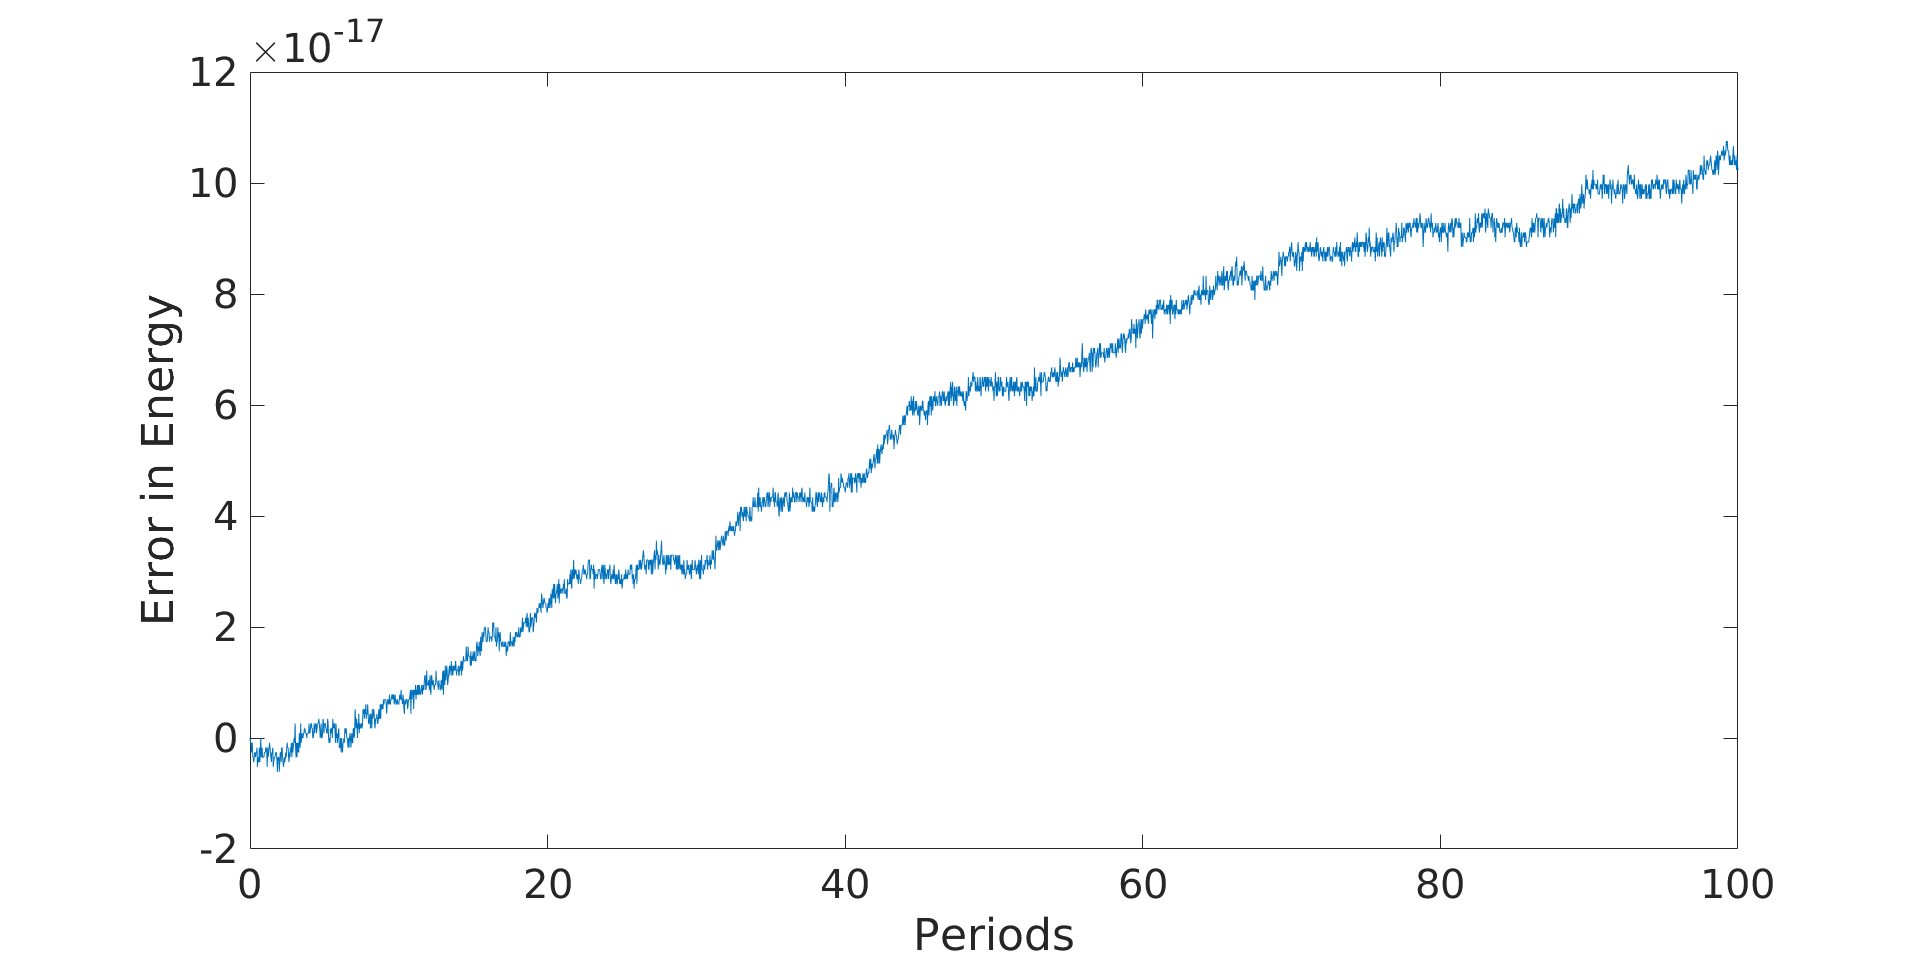
\includegraphics[width=\textwidth]{32Method0.png}
\caption{Absolute Error in Energy for the homogeneous case. Implicit Midpoint. $\Delta x = \Delta t = 1/32$.} 
\label{fig:abserrhom}
\end{figure}
\begin{figure}
\centering
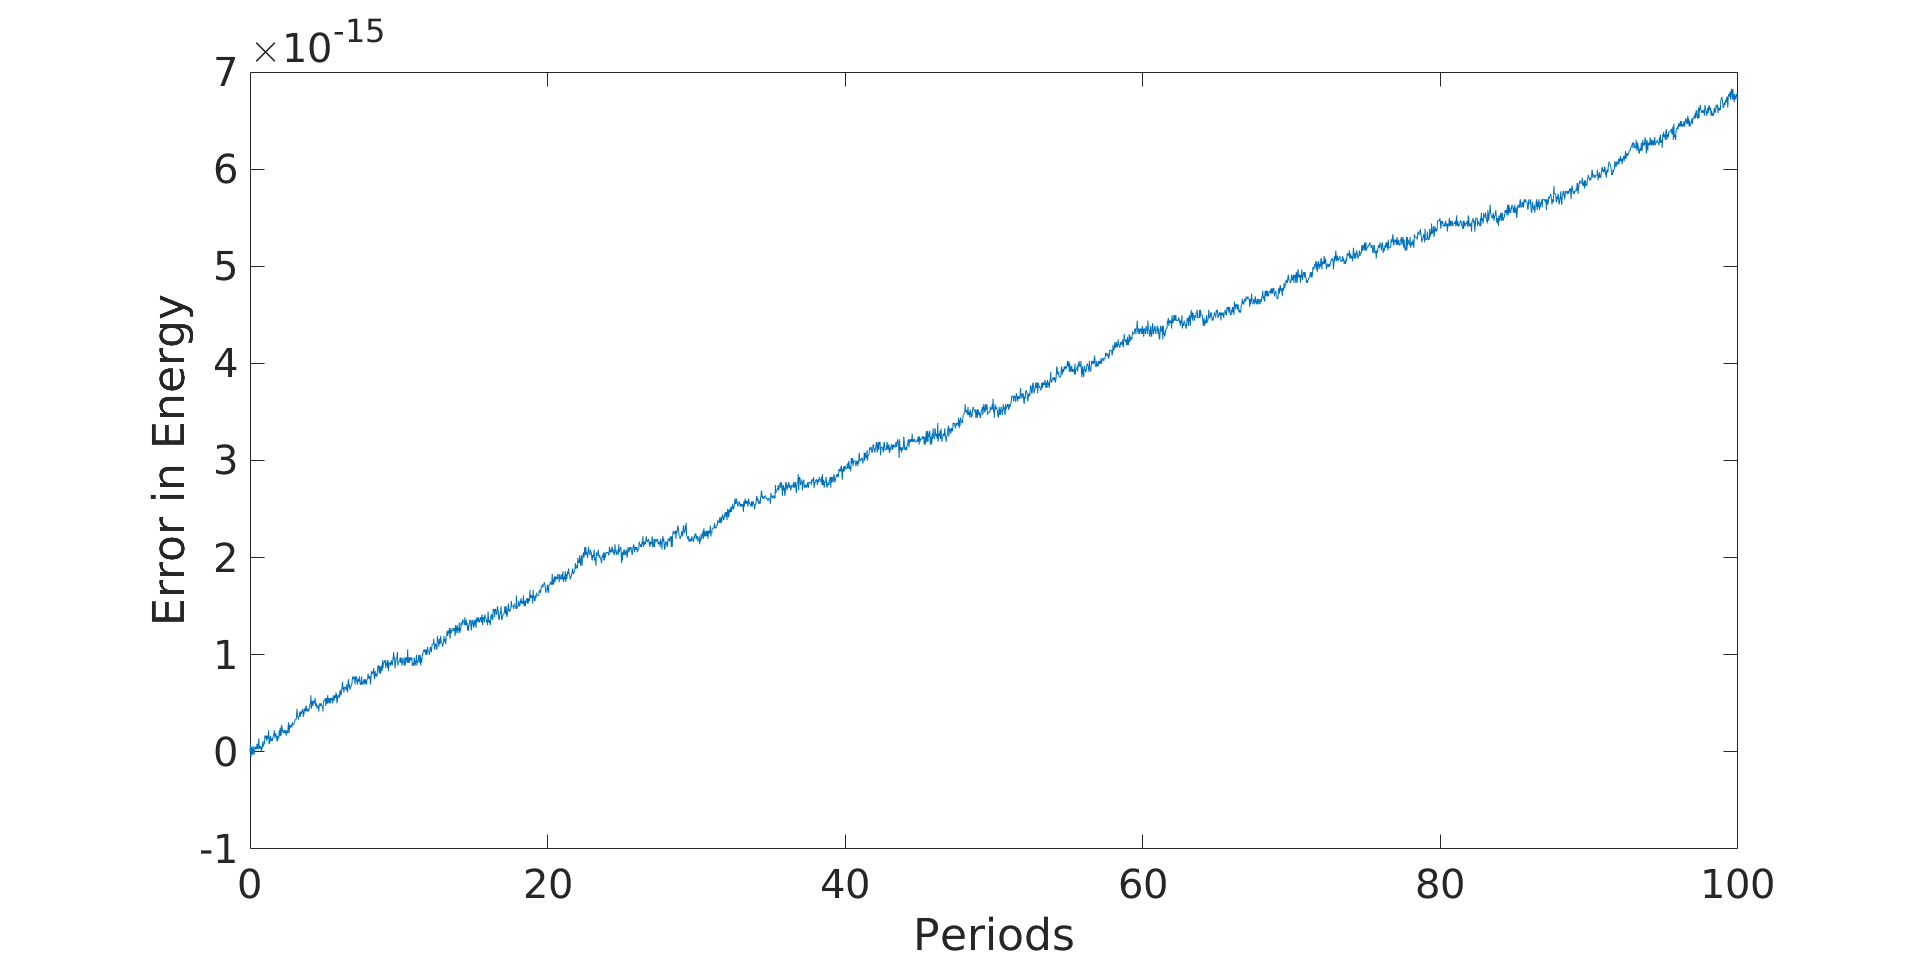
\includegraphics[width=\textwidth]{32Method1.png}
\caption{Absolute Error in Energy for the Finite Volume case. Implicit Midpoint. $\Delta x = \Delta t = 1/32$.} 
\label{fig:abserrFV}
\end{figure}
\begin{figure}
\centering
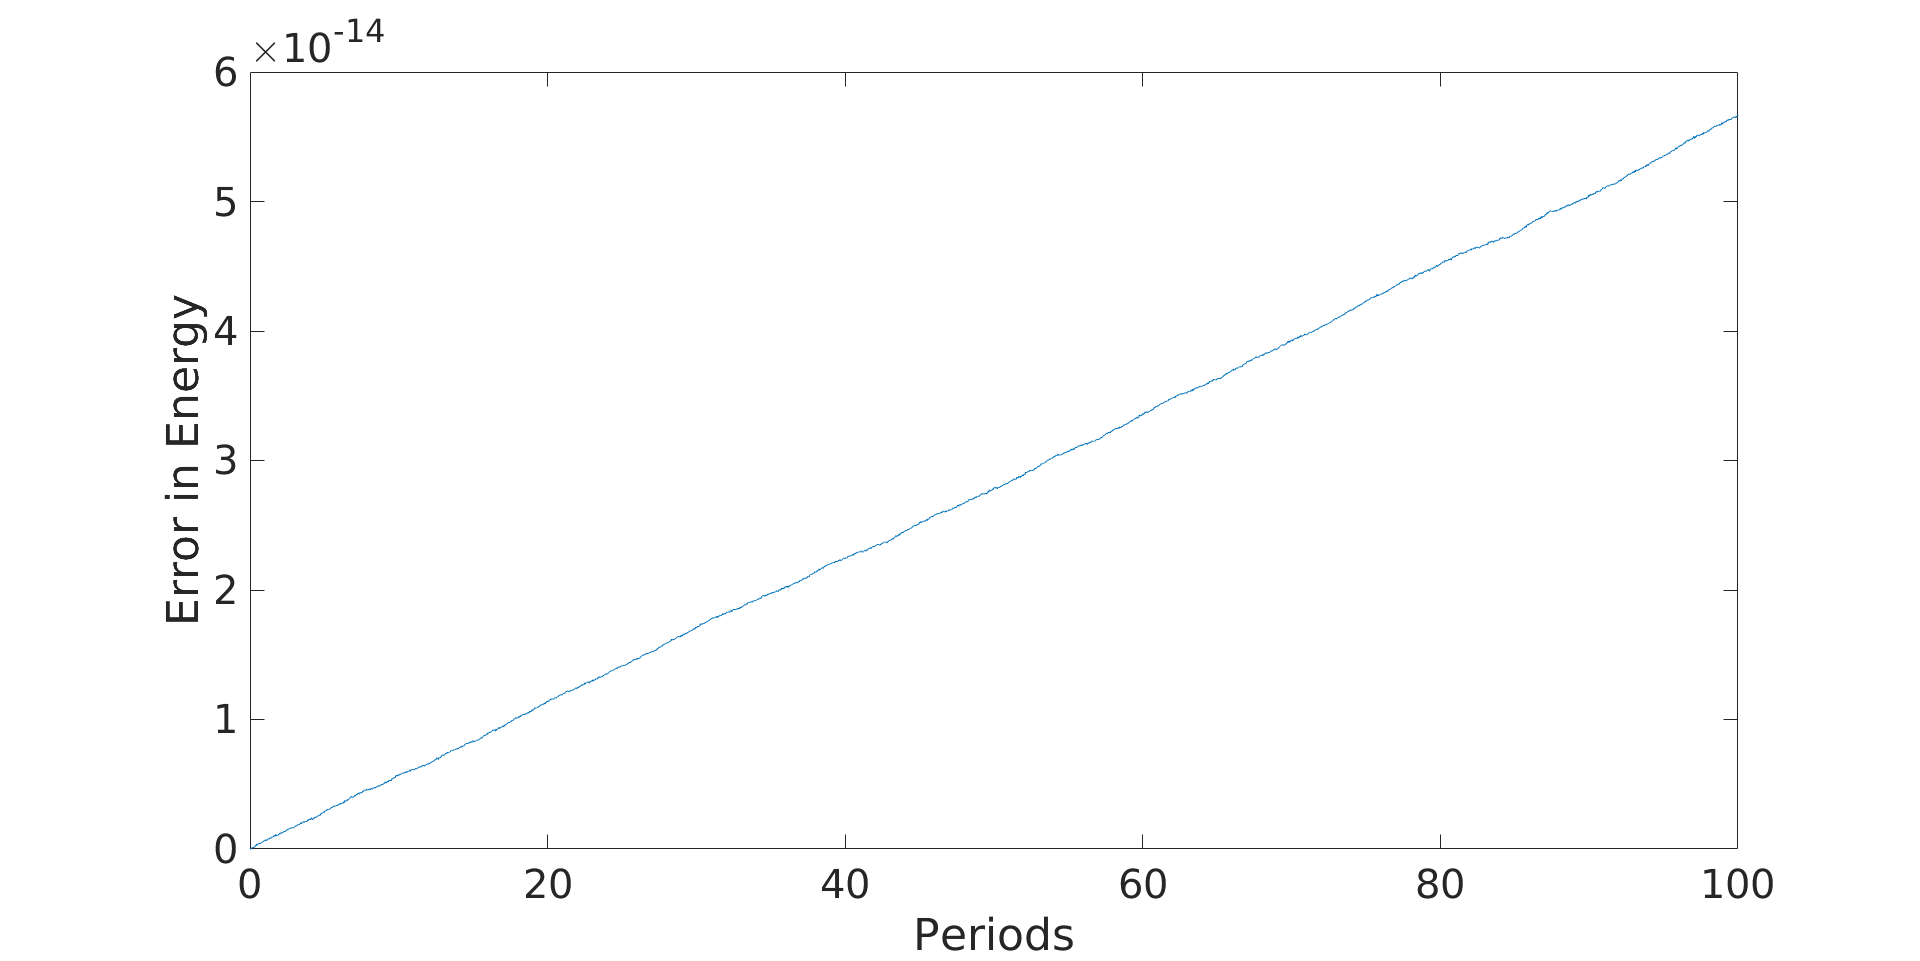
\includegraphics[width=\textwidth]{32Method2.png}
\caption{Absolute Error in Energy for the continuous case. Implicit Midpoint. $\Delta x = \Delta t = 1/32$.} 
\label{fig:abserrcon}
\end{figure}
\begin{figure}
\centering
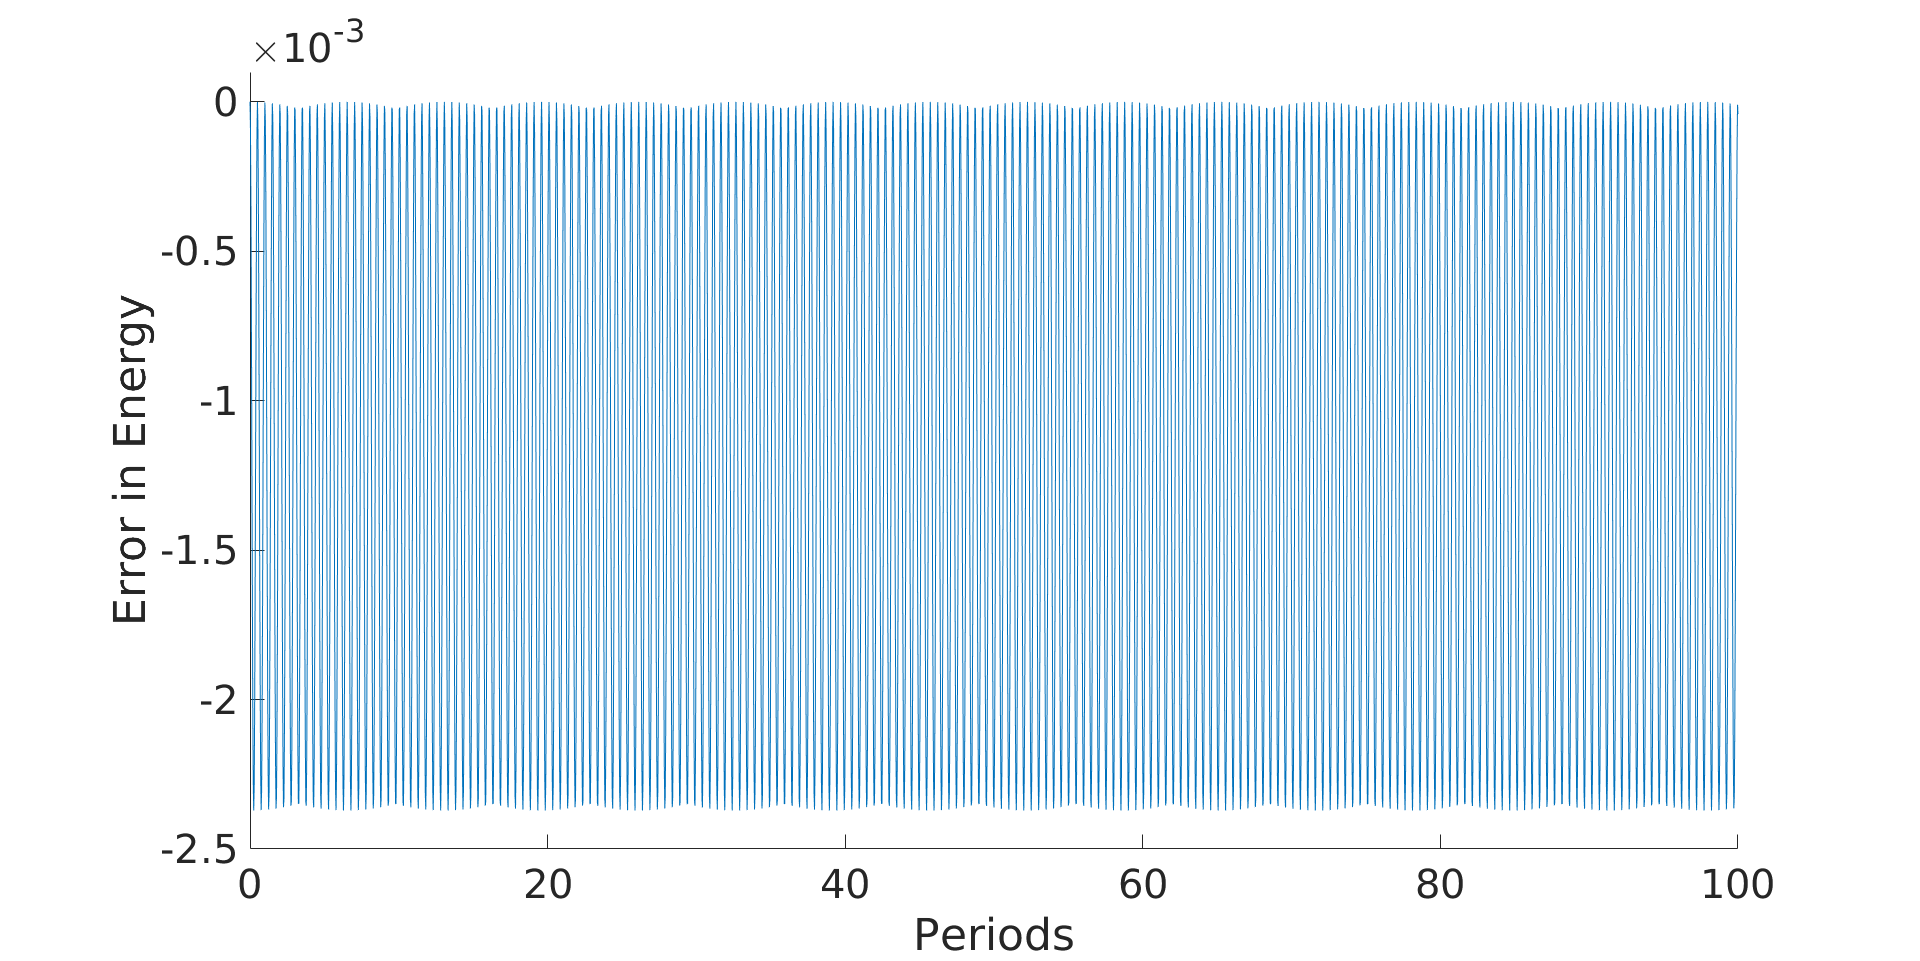
\includegraphics[width=\textwidth]{32Method4.png}
\caption{Absolute Error in Energy for the Finite Volume case. St\"{o}rmer-Verlet. $\Delta x = \Delta t = 1/32$.} 
\label{fig:abserrcon}
\end{figure}

\subsection{Conclusions}
\begin{itemize}
\item Quadrature (Simpson's Rule) and Exact Integration yielded the same results. 
\item Both replacing $\rho_0$ by a Finite Volume approximation and treating it as a continuous variable yielded energy conservation.
\item The homogeneous case and the Finite Volume case converge with an order 2, one higher than expected.
\end{itemize}
%\section{Homogeneous Viscous Test Problem}

%\subsection{Continuous Formulation}

%\subsection{Discretization}

%\subsection{Results}

%\section{Stratified Viscous Test Problem}

%\subsection{Continuous Formulation}

%\subsection{Discretization}

%\subsection{Results}

\end{document}